\documentclass[11pt,a4paper]{article}
\usepackage[T1]{fontenc}
\usepackage[margin=2.3cm]{geometry}
\usepackage{amsmath,amssymb}
\usepackage{graphicx}
\usepackage[dvipsnames]{xcolor}
\usepackage{enumitem}
\usepackage[colorlinks=true,linkcolor=blue,urlcolor=blue]{hyperref}
\setlength{\parskip}{0.6em}
\setlength{\parindent}{0pt}
\begin{document}

\begin{center}{\LARGE\bfseries openrcfilter}\\[0.4em]{\large Design a filter that removes noise from a sensor signal, in three sessions.}\\[0.2em]\small PAN IIT OSS explainer \textbullet{} secondary school to diploma / undergraduate (levels 3-5)\end{center}

\section*{Why this exists}
Every sensor signal is a mixture of what you want and what you do not. This explainer shows how a resistor and a capacitor, and then a line of code, can turn the unwanted fast part down, what that costs in delay, and how to check the result with numbers.

\section*{The end goal}
Design a filter that removes noise from a sensor signal. The end goal is to design a filter that removes noise from a sensor signal: choose the cutoff from the Bode plot, check the hum rejection in decibels, accept the delay it costs, and know when the filter fails (aliasing, a cutoff above Nyquist). The same ideas run inside audio equipment, thermostats, phones and instruments.

\section*{How the three sessions build up}
\begin{enumerate}[nosep]
\item \textbf{Session 1: A resistor and a capacitor smooth a noisy signal} (Level 1, conceptual interactive model, 60 min).
\item \textbf{Session 2: The RC low-pass in numbers: tau, cutoff, decibels and the Bode plot} (Level 2, mathematical engineering model, 75 min).
\item \textbf{Session 3: Digital filters: the exponential moving average, Butterworth and the limits} (Level 3, simulation and validation, 90 min).
\end{enumerate}

\section{Session 1: A resistor and a capacitor smooth a noisy signal}

\subsection*{A. Real-world problem}
A temperature sensor is wired to a controller across a noisy room. The reading you care about changes slowly, a couple of times per second at most, but the wire also picks up fast jitter from motors and mains cables. How can two cheap parts, a resistor and a capacitor, flatten the jitter and leave the slow signal alone? And is the result free, or does it cost us something? (General education only: this is a simplified model, not a design tool for real instruments.)

\subsection*{B. Concept and theory}
A capacitor stores charge, like a small bucket that fills and empties. A resistor in series limits how fast current can flow into the bucket. When the input voltage changes, the capacitor voltage follows it but only gradually: it moves a fixed fraction of the remaining gap towards the input in each tiny time step. The time scale of that following is the time constant tau = R C (ohms times farads gives seconds). A slow input changes little during one tau, so the output follows it. A fast wiggle reverses before the capacitor has moved far, so it is mostly ignored. That is a low-pass filter: slow gets through, fast does not. The frequency where the filter starts to ignore waves is the cutoff f\_c = 1 / (2 pi R C). The fraction of a wave of frequency f that gets through is, as a preview of Session 2, 1 / sqrt(1 + (f / f\_c)\textasciicircum{}2). The price is delay: because the capacitor lags the input, the smoothed slow wave arrives late, by roughly tau for waves much slower than f\_c.

\begin{itemize}[nosep]
\item R: resistance of the series resistor (ohm (kohm = 1000 ohm))
\item C: capacitance of the capacitor (farad (uF = 0.000001 F))
\item tau: time constant R C (seconds)
\item f\_c: cutoff frequency (hertz (Hz))
\item f: frequency of a wave in the signal (hertz (Hz))
\item gain: output size divided by input size for one wave (no unit)
\end{itemize}

\begin{equation*}
\tau = R\,C
\end{equation*}

\begin{equation*}
f_c = \frac{1}{2\pi R C}
\end{equation*}

\begin{equation*}
\text{gain}(f)=\frac{1}{\sqrt{1+(f/f_c)^2}}\qquad\text{(preview; derived in Session 2)}
\end{equation*}

\begin{equation*}
\text{delay of a slow wave}\approx \tau\quad (f\ll f_c)
\end{equation*}

\begin{center}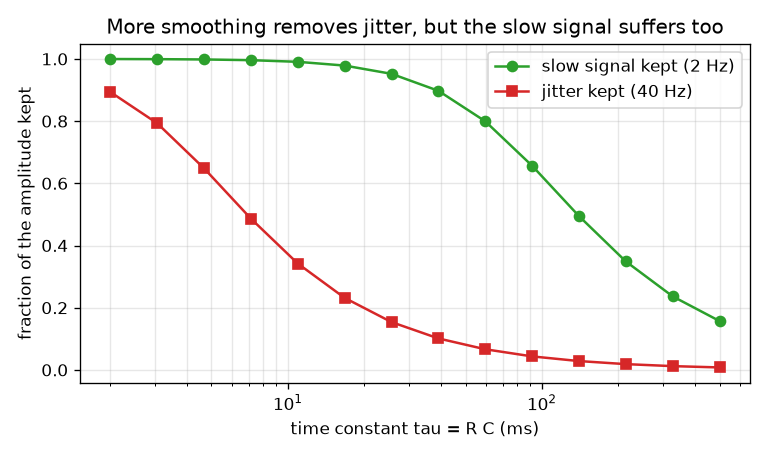
\includegraphics[width=0.85\linewidth]{figures/s01_kept_vs_tau.png}\\\small Fraction of the slow signal and of the jitter that survives, against the time constant.\end{center}

\subsection*{E. Worked example}
A filter has R = 10 kohm and C = 3.2 uF. Find tau and f\_c, how much of the 2 Hz signal and of the 40 Hz jitter get through, and how late the slow wave is.
\begin{enumerate}[nosep]
\item tau = R C = 10 000 ohm * 0.0000032 F = 0.032 s = 32 ms.
\item f\_c = 1 / (2 pi * 0.032) = 4.97 Hz.
\item Slow wave (2 Hz): f / f\_c = 0.402, gain = 1 / sqrt(1 + 0.162) = 0.928, so 92.8 percent is kept.
\item Jitter (40 Hz): f / f\_c = 8.04, gain = 1 / sqrt(1 + 64.7) = 0.123, so 12.3 percent is kept.
\item Delay of the slow wave = atan(2 / 4.97) / (2 pi * 2) = 0.3826 rad / 12.57 = 0.0304 s, about 30 ms (a little less than tau = 32 ms, as expected).
\item The simulation in lesson.py measures 0.928, 0.123 and 30.3 ms: the numbers agree.
\end{enumerate}
\textbf{Answer.} tau = 32 ms, f\_c = 4.97 Hz; the slow wave keeps 92.8 percent, the jitter keeps 12.3 percent, and the slow wave is about 30 ms late.

\subsection*{F. Questions}
\begin{enumerate}[nosep]
\item \textbf{Conceptual.} Why does an RC filter flatten fast jitter more than a slow wave? And why can it never remove the jitter without making the slow signal arrive late?
\item \textbf{Numerical.} R = 20 kohm and C = 1 uF. Find tau, f\_c, the fraction of the 2 Hz signal and of the 40 Hz jitter that is kept, and the delay of the slow wave.
\item \textbf{Graph and simulation interpretation.} Look at the figure of fraction kept against time constant. Could any single time constant keep at least 90 percent of the slow signal and at the same time let through less than 10 percent of the jitter?
\item \textbf{Design and optimisation challenge.} Design: with C = 1 uF, choose a stock resistor so that at least 90 percent of the slow signal is kept and less than 20 percent of the jitter gets through. How late is the output?
\end{enumerate}

\section{Session 2: The RC low-pass in numbers: tau, cutoff, decibels and the Bode plot}

\subsection*{A. Real-world problem}
Mains wiring leaks a 50 Hz hum into a sensor wire. An engineer picks R and C for a 100 Hz low-pass to 'remove the hum'. How many decibels of the hum does that really remove? What cutoff is needed to remove 20 dB? And what happens when the next circuit in the chain loads the filter? (A simplified model of ideal parts, for learning; not a design tool for real equipment.)

\subsection*{B. Concept and theory}
Apply a sudden 1 V step to the input. The current through R charges C, and the capacitor voltage obeys dv/dt = (1 - v) / tau, whose solution is v(t) = 1 - exp(-t / tau): 63.2 percent after one tau, 95.0 percent after three. For a sine of frequency f the output is a sine of the same frequency whose size and timing change. In complex form H = 1 / (1 + j 2 pi f R C). Its magnitude is the gain 1 / sqrt(1 + (f / f\_c)\textasciicircum{}2) and its angle is the phase -atan(f / f\_c), with f\_c = 1 / (2 pi R C). At f = f\_c the gain is 1 / sqrt(2) = 0.7071, which is -3.01 dB (half the power), and the phase is -45 degrees. Decibels are 20 log10(gain). Far above f\_c the gain is about f\_c / f, so every tenfold increase in frequency divides the gain by 10: -20 dB per decade. A Bode plot draws gain in dB (and phase) against frequency on a logarithmic axis. A load resistance R\_L across the output sits in parallel with the capacitor: the DC gain becomes R\_L / (R + R\_L) and the cutoff uses the parallel combination of R and R\_L.

\begin{itemize}[nosep]
\item tau: time constant R C (seconds)
\item v(t): capacitor voltage for a 1 V step (volts)
\item f\_c: cutoff frequency, 1 / (2 pi R C) (hertz)
\item \textbar{}H\textbar{}: gain: output amplitude over input amplitude (no unit)
\item phase: output angle relative to the input (degrees)
\item gain\_dB: 20 log10 of the gain (dB)
\item R\_L: load resistance connected to the output (ohm)
\end{itemize}

\begin{equation*}
v(t)=1-e^{-t/\tau},\qquad \tau=RC
\end{equation*}

\begin{equation*}
H(j\omega)=\frac{1}{1+j\omega RC},\qquad f_c=\frac{1}{2\pi RC}
\end{equation*}

\begin{equation*}
|H|=\frac{1}{\sqrt{1+(f/f_c)^2}},\qquad \varphi=-\arctan\!\left(\frac{f}{f_c}\right)
\end{equation*}

\begin{equation*}
\text{gain}_{\mathrm{dB}}=20\log_{10}|H|\quad\Rightarrow\quad |H(f_c)|=\tfrac{1}{\sqrt2}\;(-3.01\ \mathrm{dB}),\ \ -20\ \mathrm{dB/decade\ for}\ f\gg f_c
\end{equation*}

\begin{equation*}
\text{loaded: }\ G_0=\frac{R_L}{R+R_L},\qquad f_c'=\frac{1}{2\pi\,(R\parallel R_L)\,C}
\end{equation*}

\begin{center}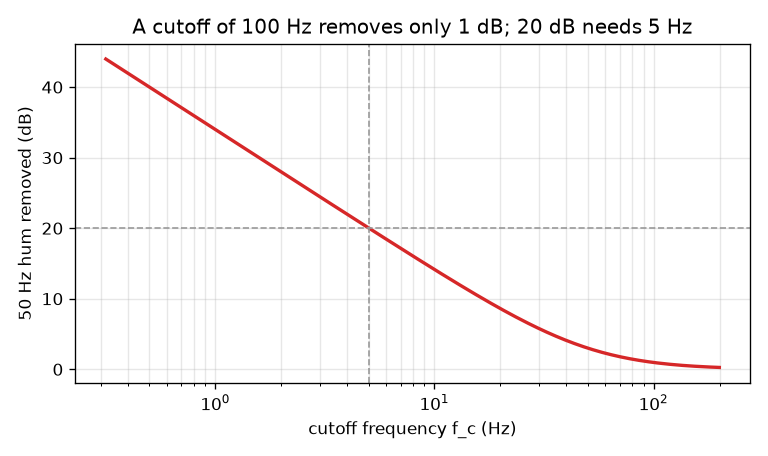
\includegraphics[width=0.85\linewidth]{figures/s02_hum_removed.png}\\\small 50 Hz hum removed (dB) against cutoff frequency: 20 dB needs about 5 Hz.\end{center}

\subsection*{E. Worked example}
Design a low-pass with f\_c = 100 Hz using C = 100 nF. Choose R (nearest E24 stock value), then compute tau, the actual cutoff, the gain at 50 Hz and how many dB of 50 Hz hum are removed. Then find the cutoff needed to remove 20 dB.
\begin{enumerate}[nosep]
\item R = 1 / (2 pi f\_c C) = 1 / (2 pi * 100 * 100e-9) = 15 915 ohm. The nearest E24 stock value is 16 kohm.
\item tau = 16 000 * 100e-9 = 1.60 ms, and f\_c = 1 / (2 pi * 0.0016) = 99.47 Hz.
\item Gain at 50 Hz: f / f\_c = 0.503, gain = 1 / sqrt(1 + 0.2528) = 0.8935.
\item In dB: 20 log10(0.8935) = -0.98 dB. So only 0.98 dB of the hum is removed: the hum is 89 percent as big as before.
\item For 20 dB we need gain 0.1: (f / f\_c)\textasciicircum{}2 = 1 / 0.1\textasciicircum{}2 - 1 = 99, so f\_c = 50 / sqrt(99) = 5.025 Hz.
\item With C = 1 uF that is R = 31.7 kohm (stock value 33 kohm, f\_c = 4.82 Hz, 20.35 dB removed, and a 1 Hz signal changes by only -0.18 dB).
\end{enumerate}
\textbf{Answer.} A 100 Hz cutoff (16 kohm, 100 nF) removes only 0.98 dB of 50 Hz hum; removing 20 dB needs f\_c = 5.025 Hz, for example 33 kohm with 1 uF (20.35 dB).

\subsection*{F. Questions}
\begin{enumerate}[nosep]
\item \textbf{Conceptual.} Why is f\_c defined at -3 dB, and what does that mean for the size of the wave and for its power?
\item \textbf{Numerical.} A filter has R = 33 kohm and C = 1 uF. Find f\_c, the dB removed from 50 Hz hum, the dB change of a 1 Hz signal and the phase at 1 Hz.
\item \textbf{Graph and simulation interpretation.} On the Bode plot of the 100 Hz filter, read the gain at 1 kHz and at 10 kHz. What does the difference tell you about the slope?
\item \textbf{Design and optimisation challenge.} Design: a sensor signal lives between 0 and 2 Hz and must not lose more than 1 dB anywhere in that band. Choose a cutoff and a stock R (with C = 1 uF) that removes as much 50 Hz hum as possible. How many dB can you remove at most, and why can you not ask for 40 dB?
\end{enumerate}

\section{Session 3: Digital filters: the exponential moving average, Butterworth and the limits}

\subsection*{A. Real-world problem}
A microcontroller samples a temperature sensor 500 times per second and cleans the numbers in software with one line of code. Does that line really behave like the RC circuit of Session 2? How much random noise does it remove, and how long must we wait for a changed temperature to show? When does it fail, and what should we use when one pole is not steep enough to remove 50 Hz hum without making the reading slow? (A simplified model for learning; real instruments need calibration and professional design.)

\subsection*{B. Concept and theory}
Sampling at rate fs means the sample time is dt = 1 / fs. The exponential moving average (EMA) is y[n] = y[n-1] + alpha (x[n] - y[n-1]). We choose alpha by exact (step-invariant) discretisation of the RC circuit: if the input is held constant during one sample, the capacitor moves exactly the fraction alpha = 1 - exp(-dt / tau) of the way to the input, so the digital step response equals 1 - exp(-t / tau) at every sample. (The common alternative, backward Euler, gives alpha = dt / (tau + dt); it is almost identical when fc is much smaller than fs.) The z-transform gives H(z) = alpha / (1 - (1 - alpha) z\textasciicircum{}-1), so the gain at frequency f is alpha / \textbar{}1 - (1 - alpha) exp(-j 2 pi f / fs)\textbar{}. It agrees with the analog gain at low frequencies but deviates near Nyquist, because the digital curve is periodic in frequency. For white noise of variance sigma\textasciicircum{}2 the output variance is sigma\textasciicircum{}2 alpha / (2 - alpha), since the impulse response h[k] = alpha (1 - alpha)\textasciicircum{}k has sum of squares alpha / (2 - alpha). A slow signal is delayed by (1 - alpha) / alpha samples, so noise power times lag equals (1 - alpha) / (2 - alpha), about 1/2: halving the noise power doubles the lag. A second-order Butterworth low-pass falls 40 dB per decade with a flat passband (Q = 1/sqrt(2)); we implement it with the standard bilinear-transform biquad (the audio-EQ cookbook low-pass) whose cutoff is pre-warped so that the -3 dB point lands exactly on fc. Sampling cannot see frequencies above fs / 2 (Nyquist): a sine of frequency f appears at \textbar{}f - fs * round(f / fs)\textbar{}. This is aliasing, and it cannot be undone in software. Also, the EMA has a -3 dB point below Nyquist only if alpha \textless{} 0.828, which for the exact alpha means fc \textless{} 0.28 fs.

\begin{itemize}[nosep]
\item fs: sample rate (hertz (samples per second))
\item dt: sample time 1 / fs (seconds)
\item alpha: EMA coefficient, 0 \textless{} alpha \textless{}= 1 (no unit)
\item x[n], y[n]: input and output at sample n (same unit as the sensor (for example C))
\item sigma\textasciicircum{}2: variance of the white noise (unit squared)
\item Q: quality factor of the biquad (1/sqrt(2) for Butterworth) (no unit)
\item fs / 2: Nyquist frequency (hertz)
\end{itemize}

\begin{equation*}
y[n]=y[n-1]+\alpha\,(x[n]-y[n-1]),\qquad \alpha=1-e^{-dt/\tau}=1-e^{-2\pi f_c/f_s}
\end{equation*}

\begin{equation*}
H(z)=\frac{\alpha}{1-(1-\alpha)z^{-1}},\qquad |H(f)|=\frac{\alpha}{\left|1-(1-\alpha)e^{-j2\pi f/f_s}\right|}
\end{equation*}

\begin{equation*}
\frac{\sigma_{\mathrm{out}}^2}{\sigma^2}=\sum_k h[k]^2=\frac{\alpha}{2-\alpha},\qquad \text{lag}=\frac{1-\alpha}{\alpha}\ \text{samples}
\end{equation*}

\begin{equation*}
\omega_0=\frac{2\pi f_c}{f_s},\ \ a=\frac{\sin\omega_0}{2Q},\ \ b_0=b_2=\frac{1-\cos\omega_0}{2(1+a)},\ \ b_1=\frac{1-\cos\omega_0}{1+a},\ \ a_1=\frac{-2\cos\omega_0}{1+a},\ \ a_2=\frac{1-a}{1+a}
\end{equation*}

\begin{equation*}
f_{\mathrm{alias}}=\left|f-f_s\,\mathrm{round}(f/f_s)\right|
\end{equation*}

\begin{center}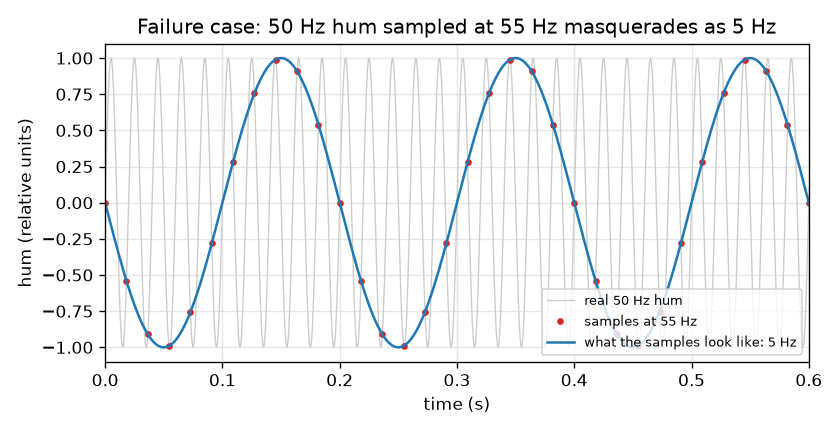
\includegraphics[width=0.85\linewidth]{figures/s03_aliasing.png}\\\small Failure case: 50 Hz hum sampled at 55 Hz looks like a 5 Hz wave.\end{center}

\subsection*{E. Worked example}
The temperature sensor is sampled at 500 Hz with an EMA of cutoff 2 Hz. Find alpha, the noise left (from 0.05 C rms), the lag, and the hum left (from 0.5 C of 50 Hz). Does it meet the limit of 0.02 C of hum? If not, try 1.5 Hz.
\begin{enumerate}[nosep]
\item alpha = 1 - exp(-2 pi * 2 / 500) = 1 - exp(-0.02513) = 0.02482.
\item Noise power factor = alpha / (2 - alpha) = 0.02482 / 1.97518 = 0.01257, so the rms noise is 0.05 * sqrt(0.01257) = 0.0056 C.
\item Lag = (1 - alpha) / alpha = 39.3 samples = 39.3 / 500 = 78.6 ms.
\item Hum: the digital gain at 50 Hz is 0.0406, so 0.5 C of hum becomes 0.0203 C. That is above the 0.02 C limit by a hair, so 2 Hz fails.
\item Try 1.5 Hz: alpha = 0.0187, hum left 0.0152 C (passes), rms noise 0.0049 C, and the simulation gives 0.244 s to reach 90 percent of the step (passes).
\end{enumerate}
\textbf{Answer.} A 2 Hz EMA at 500 Hz has alpha = 0.0248, leaves 0.0056 C of noise, lags 78.6 ms but leaves 0.0203 C of hum (just too much); 1.5 Hz leaves 0.0152 C of hum and reaches 90 percent of the step in 0.244 s.

\subsection*{F. Questions}
\begin{enumerate}[nosep]
\item \textbf{Conceptual.} The exact discretisation makes the digital step response equal the analog one at every sample. Why does the digital Bode curve still differ from the analog curve near Nyquist?
\item \textbf{Numerical.} An EMA with fc = 5 Hz is run at fs = 200 Hz. Find alpha, the noise power factor (also in dB), the lag in samples and in milliseconds, and the number of samples to reach 90 percent of a step.
\item \textbf{Graph and simulation interpretation.} From the noise-versus-lag graph, how many samples of lag are needed to cut the white-noise power by 10 dB? What does the trade-off say about halving the noise power again?
\item \textbf{Design and optimisation challenge.} Design: your microcontroller can only sample at 60 Hz, the signal band is below 1 Hz and 50 Hz hum is present. Why can a digital EMA with fc = 2 Hz not fix the hum, and what do you add? Give the hum removed and the loss of the 1 Hz signal for your solution.
\end{enumerate}

\section{Real-world mini-project}
\textbf{Design the filter for a temperature sensor with 50 Hz pickup.} A sensor reads 25.0 C and the temperature steps to 30.0 C at t = 1 s. The long wire picks up 0.5 C of 50 Hz mains hum and the electronics add white noise of 0.05 C (standard deviation); the microcontroller samples at 500 Hz. The reading must have at most 0.02 C of hum left, at most 0.008 C of random noise left, and must reach 90 percent of the step (29.5 C) within 0.5 s. Using \texttt{ema\_filter}, \texttt{butter\_filter}, \texttt{ripple\_after}, \texttt{time\_to\_90} and \texttt{noise\_rms\_after} from Session 3, scan cutoffs from 0.25 Hz to 14 Hz in steps of 0.25 Hz for both filter types.

\section{The path ahead}
\begin{enumerate}[nosep]
\item \textbf{Session 4: A notch that nulls 50 Hz.} A filter for the temperature sensor with a null at 50 Hz that is still fast.
\item \textbf{Session 5: Zero-phase filtering for recordings.} An offline filter that smooths a recorded trace without shifting it.
\item \textbf{Session 6: Anti-alias filter and decimation.} A pipeline that samples at 2000 Hz, filters, and keeps every tenth sample.
\item \textbf{Session 7: Measure a real Bode plot.} A measurement script and a breadboard filter that produce a measured Bode plot.
\item \textbf{Session 8: Reproduce the Target animation.} A looping animation of a cutoff sweep with the gain curve on one side and the noisy and filtered signals on the other.
\end{enumerate}

\section{Answers and hints}

\subsection*{Session 1}
\begin{enumerate}[nosep]
\item \textbf{Conceptual.} Hint: Think of the capacitor as a bucket that fills through a narrow pipe, and ask what happens when the input reverses before the bucket has filled. Solution: The capacitor only moves a fraction of the way towards the input in each time step. A slow wave stays on one side long enough for the output to follow it; a fast wave reverses before the output has moved far, so the output barely wiggles. The same sluggishness that ignores a fast wiggle also makes the output follow a slow change late, by about tau. A filter that ignores faster wiggles must therefore be slower to follow, so smoothing and delay always come together.
\item \textbf{Numerical.} Hint: tau = R C; f\_c = 1 / (2 pi tau); gain = 1 / sqrt(1 + (f / f\_c)\textasciicircum{}2); delay = atan(f / f\_c) / (2 pi f). Solution: tau = 20 000 * 0.000001 = 0.020 s = 20 ms. f\_c = 1 / (2 pi * 0.020) = 7.96 Hz. Slow: f / f\_c = 0.251, gain = 1 / sqrt(1.0631) = 0.970 (97.0 percent). Jitter: f / f\_c = 5.03, gain = 1 / sqrt(26.3) = 0.195 (19.5 percent). Delay = atan(0.251) / (2 pi * 2) = 0.2462 / 12.566 = 0.0196 s, about 19.6 ms. Sanity check: 20 ms is close to tau, as expected for a slow wave.
\item \textbf{Graph and simulation interpretation.} Hint: Find the f\_c needed for each wish using the gain formula, then see whether the two ranges overlap. Solution: Keeping at least 90 percent of the 2 Hz wave needs 1 / sqrt(1 + (2 / f\_c)\textasciicircum{}2) \textgreater{}= 0.9, so f\_c \textgreater{}= 4.13 Hz. Passing less than 10 percent of the 40 Hz jitter needs f\_c \textless{}= 4.02 Hz. The two ranges just miss each other (4.13 is above 4.02), so no time constant meets both wishes. The two curves in the figure indeed cross the 90 percent and 10 percent lines at slightly different places. A single RC section is not steep enough when the wanted and unwanted frequencies are only a factor 20 apart; Sessions 2 and 3 show what to do.
\item \textbf{Design and optimisation challenge.} Hint: Find the allowed range of f\_c from the two wishes, convert it to a range of R with R = 1 / (2 pi f\_c C), and pick a common value. Solution: Slow signal \textgreater{}= 90 percent needs f\_c \textgreater{}= 4.13 Hz; jitter \textless{} 20 percent needs 40 / f\_c \textgreater{} 4.90, so f\_c \textless{} 8.16 Hz. With C = 1 uF, R = 1 / (2 pi f\_c C) runs from 19.5 kohm (at 8.16 Hz) to 38.5 kohm (at 4.13 Hz). A stock value inside that range is 27 kohm: tau = 27 ms, f\_c = 5.89 Hz, slow kept 94.7 percent, jitter kept 14.6 percent, delay 26 ms. Trade-off: a larger R removes more jitter but loses more of the slow signal and arrives later.
\end{enumerate}

\subsection*{Session 2}
\begin{enumerate}[nosep]
\item \textbf{Conceptual.} Hint: Compute 10\textasciicircum{}(-3/20) and square it. Solution: At f\_c the gain is 1 / sqrt(2) = 0.7071, which is 20 log10(0.7071) = -3.01 dB. The wave amplitude is 70.7 percent of the input. Power goes with amplitude squared, so the power is exactly one half; -3 dB is the half-power point. It is a convention for 'where the filter starts to bite': the gain is already down by 29 percent there.
\item \textbf{Numerical.} Hint: f\_c = 1 / (2 pi R C); gain\_dB = -10 log10(1 + (f / f\_c)\textasciicircum{}2). Solution: f\_c = 1 / (2 pi * 33 000 * 1e-6) = 4.82 Hz. At 50 Hz: f / f\_c = 10.37, gain\_dB = -10 log10(1 + 107.5) = -20.35 dB, so 20.35 dB of hum is removed. At 1 Hz: f / f\_c = 0.207, gain\_dB = -10 log10(1.043) = -0.18 dB. Phase at 1 Hz = -atan(0.207) = -11.7 degrees. Sanity check: the hum is 10 times above f\_c, so about -20 dB, as the roll-off rule predicts.
\item \textbf{Graph and simulation interpretation.} Hint: Both frequencies are far above f\_c = 99.5 Hz. Solution: At 1 kHz the gain is about -20.1 dB and at 10 kHz about -40.0 dB. Going up by a factor 10 in frequency (one decade) lowers the gain by 20 dB: the roll-off is -20 dB per decade, a straight line on a Bode plot, because above f\_c the gain is about f\_c / f.
\item \textbf{Design and optimisation challenge.} Hint: The 2 Hz edge sets a minimum f\_c; the hum sets a maximum f\_c for a wanted attenuation. Solution: At 2 Hz the loss must be at most 1 dB: (f / f\_c)\textasciicircum{}2 \textless{}= 10\textasciicircum{}0.1 - 1 = 0.259, so f\_c \textgreater{}= 3.93 Hz. The lowest allowed cutoff gives the most hum rejection: with f\_c = 3.93 Hz the hum is down by 22.1 dB; a stock choice with margin is R = 36 kohm, C = 1 uF (f\_c = 4.42 Hz): hum removed 21.1 dB, loss at 2 Hz 0.81 dB. Asking for 40 dB would need f\_c = 0.5 Hz, which would cut the 2 Hz edge by about 12 dB. One RC section is simply not steep enough: the band edge (2 Hz) and the hum (50 Hz) are only a factor 25 apart. A steeper filter (Session 3) is the cure. Also keep the load at least 10 times R so that it does not change the gain.
\end{enumerate}

\subsection*{Session 3}
\begin{enumerate}[nosep]
\item \textbf{Conceptual.} Hint: What does a sampled system know about frequencies above fs / 2, and what is the digital gain at f and at fs - f? Solution: The digital gain is periodic in frequency: it repeats every fs, and the gain at f equals the gain at fs - f. The analog gain keeps falling as f grows, but a sampled system cannot fall forever: the curve must flatten and turn up again towards fs. Matching the step response at sample times is a time-domain statement; it does not force the frequency responses to agree everywhere. They agree well for f much smaller than fs (within 0.2 percent at fc / 2 in Figure 1) and differ near Nyquist.
\item \textbf{Numerical.} Hint: alpha = 1 - exp(-2 pi fc / fs); factor = alpha / (2 - alpha); lag = (1 - alpha) / alpha. Solution: alpha = 1 - exp(-2 pi * 5 / 200) = 1 - exp(-0.15708) = 0.1454. Noise power factor = 0.1454 / 1.8546 = 0.0784, which is 10 log10(0.0784) = -11.06 dB. Lag = 0.8546 / 0.1454 = 5.88 samples = 5.88 / 200 = 29.4 ms. Samples to 90 percent: the smallest n with 1 - (1 - alpha)\textasciicircum{}n \textgreater{}= 0.9 is n = 15 (the simulation confirms). Sanity check: the lag of about 29 ms is close to tau = 1 / (2 pi 5) = 31.8 ms.
\item \textbf{Graph and simulation interpretation.} Hint: 10 dB means a factor 0.1: solve alpha / (2 - alpha) = 0.1, then lag = (1 - alpha) / alpha. Solution: alpha / (2 - alpha) = 0.1 gives alpha = 0.2 / 1.1 = 0.1818, so lag = 0.8182 / 0.1818 = 4.5 samples. Because noise power times lag is (1 - alpha) / (2 - alpha), close to 1/2 for small alpha, halving the noise power again (another 3 dB) roughly doubles the lag. There is no free lunch: every dB of noise removed is paid for in delay.
\item \textbf{Design and optimisation challenge.} Hint: Where does 50 Hz land after sampling at 60 Hz? Then think about what must happen before the sampler. Solution: At fs = 60 Hz, Nyquist is 30 Hz and the 50 Hz hum aliases to \textbar{}50 - 60\textbar{} = 10 Hz, where it is a perfectly legal frequency that no software can tell from a real 10 Hz signal. The EMA (fc = 2 Hz, alpha = 0.189) passes the 10 Hz alias with gain 0.205 (-13.8 dB), whereas an analog filter would have cut 50 Hz by 28 dB. The fix is an analog RC anti-alias filter before the sampler, with fc = 5 Hz: it removes 20.04 dB of the 50 Hz hum and costs the 1 Hz signal only 0.17 dB. Then the digital EMA removes the remaining alias by another 13.75 dB: total hum removed 33.8 dB; the 1 Hz signal loses 0.17 + 0.97 = 1.1 dB. Better still, raise the sample rate to 500 Hz so that no aliasing happens.
\end{enumerate}

\section{How to join}
Read \texttt{CONTRIBUTING.md} in the repository, then pick an issue labelled \texttt{good first issue}. Repository: \url{https://github.com/KrunalPanchal1995/openrcfilter}

\end{document}
